% !TeX root=main.tex

\chapter{تعاریف و مفاهیم ابتدایی}
\thispagestyle{empty}

در این فصل، توضیحات مختصری در ارتباط با مفاهیم و تعاریف اولیه ارائه شده است. توضیحات ارائه شده، پیش زمینە‌ای برای فهم بهتر مسئله تشخیص موضع در شبکه‌های اجتماعی می‌باشد.

\section{شبکه‌های اجتماعی}
شبکه‌های اجتماعی
\LTRfootnote{\lr{Social Media}}
یک فناوری مبتنی بر رایانه است که قابلیت به اشتراک گذاری ایدە‌ها، افکار و اطلاعات
را از طریق شبکه‌ها و جوامع مجازی فراهم می‌کند. شبکه‌‌های اجتماعی معمولا توسط مجموعە ای از افراد شکل گرفته است که دیدگاە‌های خود را بیان کرده و در رابطه با آن تبادل نظر می‌کنند.

امروزه، بسیاری از تعاملات اجتماعی افراد در بستر شبکه‌های اجتماعی انجام می‌شود. مردم برای برقراری ارتباطات، اطلاع از اخبار و بررسی دیدگاه افراد دیگر از این رسانە‌ها استفاده می‌کنند
\cite{CAN2021101501}.
در شبکه‌های اجتماعی هر فرد می‌توانند آزادانه دیدگاه خود را مطرح کنند. همچنین از دیدگاه سایر افراد نیز مطلع می‌شود. علاوه بر همه موارد کشف دیدگاه عموم جامعه با رصد شبکه‌های اجتماعی تا حد خوبی امکان پذیر است. استفاده گروه عظیمی از کاربران از شبکه‌های اجتماعی این فرصت ر ا فراهم می‌کند تا جنبە‌های مختلف رفتار انسان از جمله موضع گیری عمومی نسبت به جنبە‌های مختلف اجتماعی و سیاسی، قابل تحلیل
باشد
\cite{ALDAYEL2021102597}.

\section{هوش مصنوعی}
هوش مصنوعی
\LTRfootnote{\lr{Artificial Intelligence}}
به فرآیند هوشمندسازی کامپیوتر برای یادگیری و تفکر گفته می‌شود. در این فرآیند هدف این است کامپیوتر همچون انسان توانایی حل مسئله و تصمیم گیری را یاد بگیرد. این اصطلاح عموما به پروژە‌هایی اطلاق می‌شود که توانایی استدلال، یادگیری از تجربیات گذشته و کشف معنا و الگو را دارند. همچنین با کمک اطلاعاتی که جمع می‌کند مکررا می‌تواند توانایی خود را بهبود دهد.

سیستم‌های توصیه‌گر
\LTRfootnote{\lr{Recommendation System}}،
دستیار هوشمند
\LTRfootnote{\lr{Intelligent Assistants}}،
موتورهای جستجو و تشخیص صدا یا دستخط از جمله کاربردهایی هستند که از دانش هوش مصنوعی استفاده می‌کنند.

\section{پردازش زبان طبیعی}
پردازش زبان طبیعی
\LTRfootnote{\lr{Artificial Intelligence}}
یکی از شاخە‌های هوش مصنوعی می‌باشد. هدف این است که کامپیوتر بتواند زبان
انسان را درک و تفسیر کند. این فرآیند شامل تبدیل گفتار به متن، آموزش مدل برای تصمیم گیری و انجام اقدامات هوشمندانه است. پردازش زبان طبیعی بر روی دادە‌های بدون ساختار کار می‌کند و به عوامل مختلفی از جمله دستور زبان، لحن و احساسات وابسته است
\cite{Chowdhary2020}.

برای درک بهتر زبان انسان توسط کامپیوتر مراحل مختلفی از جمله تحلیل واژگانی
\LTRfootnote{\lr{Lexical Analysis}}،
تحلیل نحوی
\LTRfootnote{\lr{Syntactical Analysis}}
و تحلیل معنایی
\LTRfootnote{\lr{Semantic Analysis}}
به کار گرفته می‌شود. با توجه به پیچیدە بودن فهم زبان انسان، زیر شاخه پردازش زبان طبیعی نیز یکی از پیچیدە ترین زیرشاخە‌های هوش مصنوعی در نظر گرفته می‌شود. ترجمه ماشینی
\LTRfootnote{\lr{Machine Translation}}،
حلاصه‌سازی متون
\LTRfootnote{\lr{Text Summarization}}
و تحلیل احساسات
\LTRfootnote{\lr{Sentiment Analysis}} 
از جمله کاربردهای پردازش زبان طبیعی می‌باشد. همچنین مترجم گوگل
\LTRfootnote{\lr{Google Translate}}
یکی از محبوب‌ترین ابزارهایی می‌باشد که در آن از الگوریتم‌های پردازش زبان طبیعی استفاده شده است.
\section{تعبیه کلمات}
در پردازش زبان طبیعی نمی‌توان متن را به صورت ساده و خام به عنوان ورودی به الگوریتم داد. بنابراین نیاز است کلمات در قالب بردارهای عددی قابل فهم و پردازش توسط کامپیوتر به آن وارد شوند. تعبیه کلمات~
\LTRfootnote{\lr{Machine Learning}}
به فرآیند نگاشت کلمات یا عبارات به بردارهای عددی قابل پردازش توسط کامپیوتر گفته می‌شود. این روش به طور معمول برای مدل‌سازی زبان و آمادە‌سازی متن جهت استفاده از آن در الگوریتم های پردازش زبان طبیعی استفاده می‌شود. رویکردهای مختلفی برای بازنمایی کلمات وجود دارد که در ادامه معروف‌ترین روش‌ها را مورد بررسی قرار خواهیم داد.
\begin{enumerate}
	\item کدگذاری
	\lr{one-hot}
	
	روش کدگذاری
	 \lr{one-hot}
	 سادە‌ترین و ابتدایی‌ترین روش استفاده شده برای تعبیه کلمات است. در این روش
	طول بردار تولید شده برای هر کلمه، برابر با تعداد کلمات یکتا در مجموعه دادگان مورد بررسی می‌باشد. در بردارهای تولید شده توسط این روش، یکی از درایە‌های بردار مقدار یک و بقیه درایە‌ها مقدار صفر می‌گیرند. پیادە‌سازی این روش بسیار آسان است. اما در صورت بزرگ بودن مجموعه داده، طول بردار بازنمایی کلمات بسیار بزرگ خواهد بود. همچنین عیب دیگر این روش این است که مفهومی از کلمات را در خود جای نداده است. به این دلیل که فاصله کلیه کلمات مجموعه دادگان از یکدیگر یکسان است. بنابراین بازنمایی تولید شده، فرقی مابین کلمات مترادف و یا کلمات بی ربط ایجاد نمی‌کند. در صورتی که انتظار ما این است 	فاصله بردار کلمات مترادف از یکدیگر نسبت به کلمات بی ربط به یکدیگر متفاوت باشد.
	\item کدگذاری
	\lr{TF-IDF}
	
	روش
\lr{TF-IDF}\LTRfootnote{\lr{Term Frequenct-Inverse Document Frequency}}
یکی دیگر از روش‌های مورد استفاده است. هدف از این روش، تنظیم کردن و یک دست کردن کلماتی است که بارها در متن تکرار شدە اند. متن می‌تواند شامل یک سند یا مجموعە‌ای از اسناد مختلف باشد. این روش ترکیبی از دو معیار است.
\begin{itemize}
	\item   
	\lr{TF} : 
	که عبارت است از تقسیم تعداد تکرار کلمه بر کل کلمات محتوا.
	\item   
	\lr{IDF}: 
	فراوانی سند معکوس. عبارت است از لگاریتم تقسیم تعداد کل اسناد موجود بر محتواهایی که شامل کلمه مورد نظر می‌شوند.
\end{itemize}
لازم به ذکر است
\lr{TF-IDF}
نمی‌تواند مفهوم کلمه در یک جمله را به خوبی نمایش دهد. در واقع کلمات به
بردارهایی تبدیل می‌شوند ولی توجهی به معنی کلمه در جمله نمی‌شود.

\item کدگذاری
\lr{Word2Vec}

روش
\lr{Word2Vec}\cite{41224}
یکی دیگر از روش‌های مورد استفاده برای تعبیه کلمات است. این روش کل پیکره را به عنوان ورودی می‌گیرد و کلمات را به یک بردار چند بعدی نگاشت می‌کند. بر خلاف روش
\lr{one-hot}
 در این روش بردارهای تولید شده مفاهیمی از کلمه را در خود جای دادە اند. بنابراین کلمات مشابه، بردارهای مشابه دارند. این الگوریتم دو مدل مبتنی بر شبکه عصبی ارائه  می‌دهد که در ادامه هر کدام را بررسی می‌کنیم.
 \begin{itemize}
 	\item \lr{CBOW}:
 	در این روش کلمات اطراف و نزدیک به یک کلمه به عنوان ورودی به شبکه دادە می‌شود و هر کلمه میانی به عنوان کلمه هدف در نظر گرفته می‌شود. وظیفه مدل این است با توجه به کلمات اطراف، بردار مناسب برای کلمه هدف (کلمه میانی) را تولید کند.
 	\item \lr{Skip-Gram}:
 	این روش دقیقا برعکس روش \lr{CBOW} می‌باشد. در این روش شبکه عصبی یک کلمه را به عنوان ورودی می‌گیرد و وظیفه دارد چند کلمه قبل و چند کلمه بعد از کلمه ورودی را پیشبینی کند.
 	
 \end{itemize}
\item کدگذاری
\lr{GloVe}

یکی دیگر از روش‌های تولید بردار تعبیه کلمات
\lr{GloVe}\LTRfootnote{\lr{Global Vector}}\cite{pennington-etal-2014-glove}
می‌باشد. این روش در سال ۲۰۱۴ در تیم پردازش زبان طبیعی استنفورد معرفی شده است. این روش به صورت بدون ناظر با تجمیع ماتریس هم زمانی
کلمه به کلمه سراسری 
\LTRfootnote{\lr{Global word-word co-occurrence matrix}}
 یک پیکره، یک بردار جانمایی برای هر کلمه تولید می‌کند.
 
 \item تولید بازنمایی متن با استفاده از 
 \lr{CNN ,GRU ,LSTM}
 
 با پیشرفت یادگیری عمیق در دهە‌های اخیر، پژوهشگران برای بازنمایی متن و استخراج ویژگی از شبکەهای
  \lr{CNN}\cite{kim-2014-convolutional}، \lr{LSTM} و \lr{GRU}
  نیز استفاده می‌کنند. برای استخراج ویژگی با استفاده از
 \lr{CNN}
  بردارهای کلمات در کنار یکدیگر قرار می‌گیرند. سپس به لایه پیچشی
  \LTRfootnote{\lr{Convolution Layer}}
یک بعدی داده می‌شوند و طی مراحل مختلف فیلترهای مختلفی بر روی آن‌ها اعمال می‌شود. در انتها پس از عبور از لایه
\lr{max-pooling}
ویژگی‌های مورد نظر از متن به دست می‌آید. بدین ترتیب از شبکه
 \lr{CNN}
 در پردازش زبان طبیعی برای استخراج ویژگی از متن استفاده می‌شود. شکل 
 \ref{cnn-embedding}
 فرآیند تولید بازنمایی متن با استفاده از شبکه 
  \lr{CNN} 
 را نشان می‌دهد. برای تولید بازنمایی متن توسط LSTM و GRU کافیست جمله (عبارت) مورد نظر به عنوان ورودی به شبکه داده شود. خروجی آخرین گام زمانی به عنوان بازنمایی جمله (عبارت) ورودی در نظر گرفته می‌شود.
 
 \begin{figure}[H]
 	\center{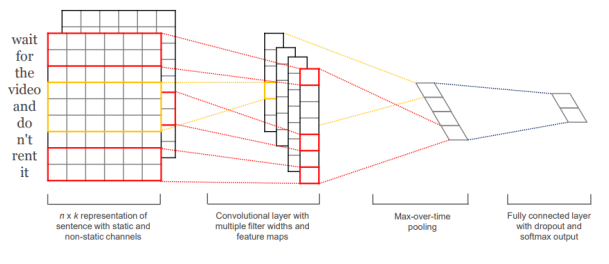
\includegraphics[width=0.6\linewidth]{images/cnn_embedding.PNG}}
 	\caption[تولید بازنمایی متن با استفاده از شبکه
 	\lr{CNN}]{تولید بازنمایی متن با استفاده از شبکه
  \lr{CNN}\cite{kim-2014-convolutional}	
 }
 	\label{cnn-embedding}
 \end{figure}
 \item کدگذاری
 \lr{BERT}
 
 
 مدل 
  \lr{BERT} \cite{devlin-etal-2019-bert}
در سال ۲۰۱۹ توسط گوگل معرفی شد.
\lr{BERT}
 یک مدل از پیش آموزش دیده برای مسائل پردازش زبان طبیعی می‌باشد. از این مدل برای تولید بازنمایی متن با کیفیت بالا می‌توان استفاده کرد. به دلیل اینکه شبکه  \lr{BERT} بر روی حجم بسیار داده آموزش دیده، بازنمایی بهتری از کلمه تولید می‌کند. همچنین با آموزش مجدد لایه آخر، برای وظایف متفاوت قابل استفاده است. مدل \lr{BERT} مبتنی بر ترنسفورمر و شامل رمزگذار دو طرفه عمیق می‌باشد.
 
 
 انواع دیگری از مدل‌های مبتنی بر
  \lr{BERT}
  نیز معرفی شدند. مدل 
 \lr{RoBERTa}\cite{liu2019roberta}
 با الگوگیری از مدل
 \lr{BERT}
 آموزش دیده است. تفاوت اصلی 
 \lr{RoBERTa}
 با
 \lr{BERT}
 در ابرپارامترهای استفاده شده است. در \lr{RoBERTa}
 اندازه دسته و نرخ یادگیری بزرگ‌تر می‌باشد. برخلاف
 \lr{BERT}
  در آموزش اولیه
 \lr{RoBERTa}
از مسئله
\lr{next-sentence prediction}
استفاده نمی‌شود. مدل
  \lr{BERTweet}\cite{bertweet}
  با روش آموزشی 
  \lr{RoBERTa}
بر داده‌های توییتر انگلیسی آموزش دیده است.  \lr{DEBERTA}\cite{liu2019roberta}
مدل
 \lr{BERT}
 و
 \lr{RoBERTa}
را با کمک توجه از هم گسسته، بهبود می‌بخشد.
\lr{XLM-RoBERTa}\cite{conneau2019unsupervised}
یک مدل چندزبانه است که بر داده‌های
\lr{CommonCrawl}
آموزش دیده است. 

\end{enumerate}

\section{یادگیری ماشین}
یادگیری ماشین
\LTRfootnote{\lr{Machine Learning}}
یکی از شاخە‌های مهم هوش مصنوعی می‌باشد. در این روش هدف یادگیری یک مدل ریاضی با استفاده از دادە‌های موجود به جای تعیین صریح قوانین در مسئله می‌باشد. بنابراین از الگوریتم‌هایی برای یادگیری الگوها و هم بستگی‌های موجود در داده‌ها استفاده می‌شود. در نهایت با استفاده از الگوهای به دست آمده یک مدل ریاضی تعریف می‌شود که از آن برای تصمیم گیری و پیشبینی استفاده می‌شود. هر چه به دادە‌های بیشتری دسترسی داشته باشیم، الگوهای بهتر و مطمئن‌تری از دادە‌ها استخراج کرده و بنابراین پیشبینی‌های دقیق‌تری خواهیم داشت.


\section{یادگیری عمیق}
یادگیری عمیق
\LTRfootnote{\lr{Deep Learning}}
شاخە‌ای از یادگیری ماشین است که مبتنی بر شبکە‌های عصبی مصنوعی
\LTRfootnote{\lr{Artificial Neural Networks}}
می‌باشد. فرآیند یادگیری، عمیق نامیده می‌شود چرا که از چندین نورون ورودی و خروجی و چندین لایه پنهان ساخته شده است.

در حالی که الگوریتم‌های یادگیری ماشین قادر هستند بسیاری از مسائل پیچیده را حل کنند، اما همچنان در برخورد با دادە‌های غیرساختاری از جمله متن، عکس و فیلم عملکرد ضعیفی دارند. روش‌های یادگیری عمیق با استفاده از شبکه‌های عصبی عمیق (که یک نوع معماری الهام گرفته از مغر انسان می‌باشد)، این مشکل را حل می‌کنند. هر لایه از شبکه عمیق ویژگی‌هایی از دادە‌های ورودی استخراج می‌کند که در نهایت می‌توان توسط ویژگی‌های استخراج شده، مسئله مورد نظر را حل کرد. اطلاعات ورودی از طریق لایە‌ها به
جلو حرکت می‌کند. 
\iffalse
در شکل
\ref{ann}
معماری یک شبکه عصبی عمیق نمایش داده شده است. در این شکل لایه ورودی، لایە‌های پنهان و لایه خروجی نیز نمایش داده شده است.

\begin{figure}[H]
	\center{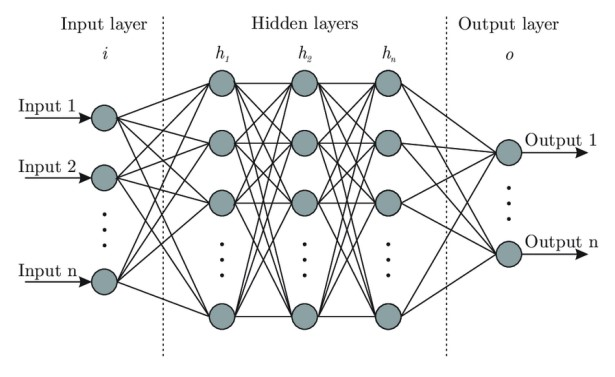
\includegraphics[width=0.5\linewidth]{images/ANN.jpg}}
	\caption{نمونه‌ای از شبکه عصبی عمیق}
	\label{ann}
\end{figure}
\fi

\section{شبکه‌های عصبی همگشتی}
شبکه‌های عصبی بازگشتی
\LTRfootnote{\lr{Recurrent Neural Network (RNN)}}
نوعی از شبکه عصبی مصنوعی است که در تشخیص گفتار، پردازش زبان طبیعی، پردازش دادە‌های ترتیبی
\LTRfootnote{\lr{Sequential Data}} 
و داده‌های سری زمانی
\LTRfootnote{\lr{Time Series}}
مورد استفاده قرار می‌گیرد. معماری این شبکه به گونە‌ای است که امکان ذخیره اطلاعات قبلی را در خود فراهم می‌کند. در بسیاری از شبکە‌های عمیق مانند شبکه عصبی پیشخور
\LTRfootnote{\lr{Feedforward Neural Network}}
دادە‌ها در یک جهت حرکت می‌کنند. یعنی از لایه ورودی به لایە‌های پنهان و سپس به سمت لایە خروجی حرکت می‌کنند و دادە‌های قبلی به حافطه سپرده نمی‌شوند. در حالی که شبکە‌های عصبی بازگشتی یک لایه بازخورد دارند که خروجی شبکه به همراه ورودی جدید، به شبکه وارد می‌شوند. این شبکه‌ها اطلاعات مربوط به ورودی قبلی را برای تاثیر بر روی ورودی و خروجی فعلی در حافظه خود ذخیره می‌کنند. در حالی که در شبکە‌های عصبی عمیق خروجی‌های مختلف از یکدیگر مستقل هستند، خروجی شبکه عصبی بازگشتی علاوه بر ورودی فعلی به عناصر قبلی توالی نیز وابسته است.

مشکل اصلی شبکە عصبی بازگشتی حافظه کوتاه مدت آن است. در بلند مدت این شبکه توانایی نگهداشتن اطلاعاتی که در گام‌های زمانی بسیار قبل‌تر به عنوان ورودی به شبکه داده شدە است را ندارد. علت این مشکل پدیده محو شدگی گرادیان
\LTRfootnote{\lr{Vanishing Gradient}}
می‌باشد. این پدیده بیان می‌کند در فرآیند بازگشت خطا به عقب
\LTRfootnote{\lr{Backpropagation}}
زمانی که به ابتدا شبکه می‌رسیم، گرادیان به تدریج کوچک می‌شود. در نتیجه تغییرات وزن بسیار کند و ناچیز می‌شود و
به عبارت دیگر آموزش کند می‌شود. این مسئله معمولا به خاطر عمق زیاد شبکه اتفاق می‌افتد. معماری‌های دیگری از جمله  \lr{LSTM} 
\cite{6795963}
و \lr{GRU} 
\cite{69e088c8129341ac89810907fe6b1bfe}
برای رفع این مشکل پیشنهاد شده است. 

ویژگی متمایز \lr{LSTM}
\LTRfootnote{\lr{Long Short-Term Memory}}
 قابلیت یادگیری وابستگی بلند مدت است که توسط شبکە‌های عصبی بازگشتی امکان پذیر نبود. شبکه عصبی بازگشتی تنها قادر به یادگیری تعداد محدودی از وابستگی‌های کوتاه مدت بود. برخلاف شبکه عصبی بازگشنی که در آن محتوا در هر گام از ابتدا بازنویسی می‌شود، در معماری \lr{LSTM} شبکه قادر است در یک گام زمانی محتوا حافظه را بدون تغییر به گام بعدی منتقل کند. به عنوان مثال اگر در گام‌های ابتدایی شبکه اطلاعات مهمی را تشخیص دهد، می‌تواند آن را برای گام‌های طولانی بدون تغییر در حافظه خود ذخیره کند.

معماری \lr{GRU} 
\LTRfootnote{\lr{Gated Recurrent Unit (GRU)}}
در سال ۲۰۱۴ معرفی شد. معماری \lr{GRU} نسخه ساده شده \lr{LSTM} می‌باشد. \lr{GRU} علاوه بر رفع مشکل محو شدگی گرادیان در شبکە عصبی بازگشتی، سربار محاسباتی \lr{LSTM} را نیز کاهش می‌دهد. همچنین با کم کردن تعداد دروازە‌ها، سرعت محاسبات را افزایش داده است.
\section{ساز و کار توجه
}\label{attention}
هدف استفاده از ساز و کار توجه
\LTRfootnote{\lr{Attention}}
بازیابی اطلاعات از بردارهای زمینه
\LTRfootnote{\lr{Context Vector}}
\lr{${y_j}$}
در رابطه با بردار پرس‌وجو
\LTRfootnote{\lr{Query Vector}}
\lr{$x$}
می‌باشد. ساز و کار توجه ابتدا امتیاز 
\lr{$\alpha_j$}
را بین بردار پرس‌وجو 
\lr{$x$}
و بردار زمینه
\lr{$y_j$}
محاسبه می‌کند.
\begin{equation}
	a_j = Score(x, y_j)
\end{equation}
\begin{equation}
	\alpha_j = \frac{exp(a_j)}{\sum_{k} exp(a_k)}
\end{equation}
خروجی لایه توجه میانگین وزن‌دار امتیاز 
\lr{$\alpha_j$}
به ازای بردار‌های زمینه می‌باشد. محاسبات انجام شده مشابه لایه 
\lr{softmax}
است. اگر بردار پرس‌وجو
\lr{$x$}
مجموعه‌ای از بردار زمینه
\lr{$\{y_j\}$}
باشد، امتیاز به دست آمده از معادله
\ref{self}
توجه به خود\LTRfootnote{\lr{self-attention}}
نامیده می‌شود.
\begin{equation}\label{self}
	Att_{x \to \{y_j\}} = \sum_{j} \alpha_jy_j
\end{equation}


\section{ترنسفورمر}
ترنسفورمر
\cite{NIPS2017_3f5ee243}
، جدیدترین معماری معرفی شده برای مسائل پردازش زبان طبیعی می‌باشد. این معماری
در سال ۲۰۱۷ معرفی شد. ترنسفورمرها با استفاده از مکانیزم توجه، امکان پردازش موازی دادە‌ها را فراهم می‌کنند. با استفاده از ترنسفورمرها برای هر کلمه می‌توان بردار بازنمایی تولید کرد. همچنین به دلیل آموزش موازی، سرعت آموزش نیز بهبود قابل توجهی پیدا می‌کند. ترنسفورمرها این قابلیت را برای ما فراهم می‌کند که به جای پردازش دنباله ورودی از ابتدا تا انتها، تنها به قسمت‌های مهم توجه کنیم. این مدل ها معمولا بر روی حجم بالایی از دادە‌ها از پیش آموزش می‌بینند
\LTRfootnote{Pre-train}.

مدل‌های زبانی بزرگ
\LTRfootnote{\lr{Large Language Models (LLMs)}}
دسته‌ای از مدل‌های زبانی هستند که توانایی درک و تولید متنی شبیه انسان را دارند. این مدل‌ها معمولاً شامل میلیون‌ها تا میلیاردها پارامتر قابل آموزش می‌باشند. برخی از آن‌ها با معماری مبتنی بر ترنسفورمرها ساخته شده‌اند.
\lr{LLMs}
ها بر روی میلیون‌ها داده آموزش دیده‌اند تا بتوانند تا بتوانند زبان انسان و انواع دیگر داده‌های پیچیده را تفسیر کنند. برخی از معروف‌ترین مدل‌های زبانی بزرگ شامل
\lr{GPT-3}،
\lr{LLaMA}\cite{touvron2023llama}
و 
\lr{Orca}\cite{orca-mini-v3-7b}
می‌باشند. 
\lr{Orca}
یک نمونه از مدل زبانی کوچک است که در دو نسخه 7 میلیارد و 13 میلیارد پارامتری عرضه شده است. این مدل با 
\lr{fine-tuning}
مدل 
\lr{LLaMA}
بر داده‌های مصنوعی با کیفیت بالا ایجاد شده است.

\section{مهندسی پرامپت}
پرامپت یک دستور متنی است که وظیفه‌ مدل را توصیف می‌کند. جدول
\ref{prompt-example}
نمونه‌‌ای از دستور متنی برای رده‌بندی در مسئله تحلیل احساسات را نشان می‌دهد (بخش‌های مختلف پرامپت نیز مشخص شده است).
\begin{table}[h!]
	\centering
	\caption{نمونه پرامپت برای مسئله تحلیل احساسات	\label{prompt-example}}
	\begin{tabular}{c c  c}
		
		دستورالعمل &  ورودی & خروجی
		\\
		\hline
		
		\lr{Classify the text into neutral, negative, or positive.}
		& \lr{Text: I think the food was okay.} 
		& \lr{Sentiment:}
	\end{tabular}

\end{table}

مهندسی پرامپت
\LTRfootnote{\lr{Prompt ٍEngineering}}
توسعه و بهینه‌سازی پرامپت برای استفاده کارآمد از مدل‌های زبانی بزرگ است. این مهارت شامل طراحی یک ورودی (دستورالعمل) مناسب برای 
\lr{LLMs} 
می‌باشد به گونه‌ای که مدل بتواند بهترین خروجی را تولید کند. مهندسی پرامپت با یادگیری درون متنی
\LTRfootnote{In-context learning}
معنا پیدا می‌کند. منظور از یادگیری درون متنی این است که مدل توانایی یادگیری موقت از پرامپت را داشته باشد. برای طراحی یک پرامپت کارآمد رویکردهای متفاوتی وجود دارد که در ادامه معروف‌ترین رویکردها را معرفی می‌کنیم
\LTRfootnote{\href{https://www.promptingguide.ai/}{https://www.promptingguide.ai/}}.

\begin{enumerate}
	\item رویکرد \lr{Zero-Shot}: 
در این رویکرد فقط یک دستورالعمل به مدل داده می‌شود (مشابه جدول 
\ref{prompt-example}). 
	\item رویکرد \lr{Chain of thought}:
	این رویکرد توانایی استدلال پیچیده را از طریق استدلال میانی برای مدل فراهم می‌کند. اضافه کردن 
	\lr{"Let's think step by step"}
	به انتهای متن یکی از معمول‌ترین دستورالعمل‌های این تکنیک به حساب می‌آید.

	\item رویکرد \lr{Few-Shot}:
	در این رویکرد علاوه بر دستورالعمل برای انجام مسئله تعریف شده، تعدادی مثال‌ از ورودی و خروجی مطلوب نیز در پرامپت گنجانده می‌شود. 
\end{enumerate}

\section{جستجو پارامترها}
مدل‌های یادگیری ماشین شامل پارامترها و فراپارامترهایی
\LTRfootnote{Hyperparameter}
 هستند که می‌توانند مقادیر مختلفی داشته باشند. انتخاب مقادیر این پارامترها همواره یکی از چالش‌های یادگیری به حساب می‌آید. روش‌های مختلفی برای انتخاب پارامترها وجود دارد. ساده‌ترین رویکرد برای انتخاب پارامترها  جستجو تصادفی
\LTRfootnote{Random Search}
می‌باشد. در این رویکرد برای هر یک از پارامترها یک فضا جستجو تعریف می‌شود. در هر بار اجرا به صورت کاملا تصادفی برای هر پارامتر مقداری انتخاب می‌شود. این روش لزوما بهترین مقادیر را هر پارامتر را به دست نمی‌آورد.
روش جستجو شبکه‌ای 
\LTRfootnote{Grid Search}
تمام حالت‌های ممکن فضا تعریف شده را جستجو می‌کند. مشکل اصلی این روش نفرین ابعاد
\LTRfootnote{Curse of Dimensionality}
می‌باشد. به این معنی که هر چه ابعاد فضا جستجو بزرگ‌تر شود، پیچیدگی زمانی به صورت نمایی افزایش پیدا خواهد کرد.


برخی از روش‌های بهینە‌سازی فراپارامترها در هر بار انتخاب فراپارامترها برای آزمایش بعدی، از اطلاعات ترکیب قبلی نیز استفاده می‌کنند. این روش‌های انتخاب تطبیقی
\LTRfootnote{Adaptive Selection}،
با انتخاب فراپارامترهایی که احتمال موفقیت‌شان بیشتر است، سرعت جستجو را به طور قابل توجهی افزایش می‌دهند. یکی از ابزارهای معرفی شده در این روش،
\lr{Optuna}\cite{10.1145/3292500.3330701}
می‌باشد. این رویکرد فضا جستجو پارامترها را به صورت پویا ساختاردهی می‌کند. برای انتخاب هر نمونه از فصا جستجو از الگوریتم
\lr{TPE}\LTRfootnote{Tree-Structured Parzen Estimator}
که بر مبنای بهینه‌سازی
\lr{Bayesian}
است استفاده می‌کند. همچنین 
\lr{Optuna}
با قابلیت توقف زود هنگام
\LTRfootnote{Early Stopping}
با استفاده از روش‌های 
\lr{Pruning}
احتمال رسیدن به پارامترهای بهینه در کوتاه‌ترین زمان ممکن را افزایش می‌دهد.

\section{جمع بندی}
در این فصل، ابتدا شبکه اجتماعی و پردازش زبان طبیعی معرفی شد. سپس مکانیزم‌های تعبیه کلمات که یکی از مهم‌ترین روش‌های کار با متن است مورد بررسی قرار گرفت. همچنین مفاهیم یادگیری عمیق، مهندسی پرامپت و روش‌های جستجو به عنوان مهم‌ترین رویکرد حل مسئله بررسی شد. آشنایی با این مفاهیم، درک مسئله تشخیص موضع را آسان تر می‌کند.
	


